\fancychapter{Introduction}
\cleardoublepage%
% The following line allows to ref this chapter
\label{chap:intro}%



\section{Motivation}
 
% \par Worldwide, there has been growing interest in the use of autonomous vehicles to execute missions of increasing complexity without constant supervision of human operators.~\cite{xargay2012time} A key-enabling element for the execution of such missions is the availability of advanced methods for cooperative motion planning that take explicitly into account temporal and spatial constraints, intrinsic vehicle limitations and energy minimisation requirements. 
% \par Some autonomous vehicle applications require groups of robots acting cooperatively. An application example that will greatly benefit from vehicle cooperation and that will be focus of this thesis is the control of groups of \acp{AUV} where the visibility is low and obstacles are not known in advance. The \acp{AUV} that together form a robot formation, can, for example, adapt better to unforeseen circumstances in the terrain by making better use of the larger environments that they can observe as the spatial distance between each \ac{AUV} can be varied.
% \par This project has evolved from earlier investigations on underwater mapping connected with the European R\&D Project "MORPH" Project~\cite{morph,aguiar2009cooperative,abreu2016widely} that Insitituto Superior Técnico was a part of. Figure~\ref{fig:morph} illustrates \acp{AUV} in operation on the Morph project.

% \par Worldwide, there has been growing interest in the use of autonomous vehicles to execute missions of increasing complexity without constant supervision of human operators.~\cite{xargay2012time} A key-enabling element for the execution of such missions is the availability of advanced methods for cooperative motion planning that take explicitly into account temporal and spatial constraints, intrinsic vehicle limitations and energy minimisation requirements. 
% \par Some autonomous vehicle applications require groups of robots acting cooperatively. An application example that will greatly benefit from vehicle cooperation and that will be focus on this thesis is the control of groups of \acp{AUV} where the visibility is low and obstacles are not known in advance. The \acp{AUV} that together form a robot formation, can, for example, adapt better to unforeseen circumstances in the terrain by making better use of the larger environments that they can observe as the spatial distance between each \ac{AUV} can be varied.
% \par This project has evolved from earlier investigations on underwater mapping connected with the European R\&D Project "MORPH" Project~\cite{morph,aguiar2009cooperative} and the "WiMUST" Project~\cite{abreu2016widely} that Insitituto Superior Técnico was a part of. Figure~\ref{fig:morph} illustrates \acp{AUV} in operation on the Morph project.
% \par The "WiMUST" project, in particular, was composed by a small fleet of \acp{AUV} towing streamers with hydrophones to acquire sub-bottom profiling acoustic data.
% \par Recent advancements on the usage of \textit{Bernstein Polynomials} for control also appear to be advantageous,~\cite{cichella2018bernstein}, shows that it's possible to control a high number of vehicles with small computation time.



\par Worldwide, there has been growing interest in the use of autonomous vehicles to execute missions of increasing complexity without constant supervision of human operators. 
\par The WiMUST project \cite{sonar_tec_overview} is an example of a project that demanded the use of such autonomous vehicles. The goal of the WiMUST project was to design a system of cooperating \acp{AUV} able to perform innovative geotechnical surveying operations. Specifically, the WiMUST system consisted of an array of physically disconnected \acp{AUV}, acting as intelligent sensing and communicating nodes of a moving acoustic network. Together, the vehicles form a geometry formation which is actively controllable according to the needs of a specific application. 
\par Applications for the \ac{AUV} formation handled by the WiMUST system include seabed mapping, seafloor characterization and seismic exploration. The overall system behaves as a distributed acoustic array capable of acquiring acoustic data obtained by illuminating the seabed and the ocean sub-bottom with strong acoustic waves sent by one (or more) acoustic sources installed onboard a support ship/boat (see figure \ref{fig:WiMUST_System}). Advantages of multiple \acp{AUV} acting cooperatively as opposed to a single one include robustness against failure of a single node and improving the seabed and sub-bottom resolution. They can also adapt better to unforeseen circumstances in the terrain by making better use of the larger environments that they can observe as the spatial distance between each \ac{AUV} can be varied. 
\par Another, unrelated, example of application that justifies the use of multiple autonomous vehicles was the Intel show at the 2018 Winter Olympics, where 1200 drones were used to put on a light show in the night sky. Each drone was mounted with a light bulb and, together, formed different shapes in the sky.
\par Complex systems like the two previously presented have in common the ability to properly plan motion for each vehicle that satisfies certain criteria such as simultaneous arrival of each vehicle in a formation while minimizing spent energy or time and avoiding collisions between vehicles and the environment.
\par Over the past decades, many approaches to solve motion planning problems have been proposed. Examples include bug algorithms, randomised algorithms such as PRM, RRT, RRT*, cell decomposition methods, graph-based approaches, planners based on learning, and methods based on optimal control formulations. Each technique has different advantages and disadvantages, and is best-suited for certain types of problems. Trajectory generation based on optimal control formulations stands out as particularly suitable for applications that require the trajectories to minimize (or maximize) some cost function while satisfying a complex set of vehicle and problem constraints. Finding closed-form solutions for Optimal Control problems can be difficult or even impossible to solve, and therefore numerical solutions must be sought. A numerical alternative to solve such complex Optimal Control problems consists in optimising trajectories given by Bernstein Polynomials. \todo{see this sentence} Recent pioneering work on the use of Bernstein Polynomials \cite{lorentz2013bernstein} for the numerical approximation of these Optimal Control problems show interesting results \cite{cichella2018bernstein}, namely, they show how can  which will be further explored in the work of this thesis.

\begin{figure}[h!]
    \centering
    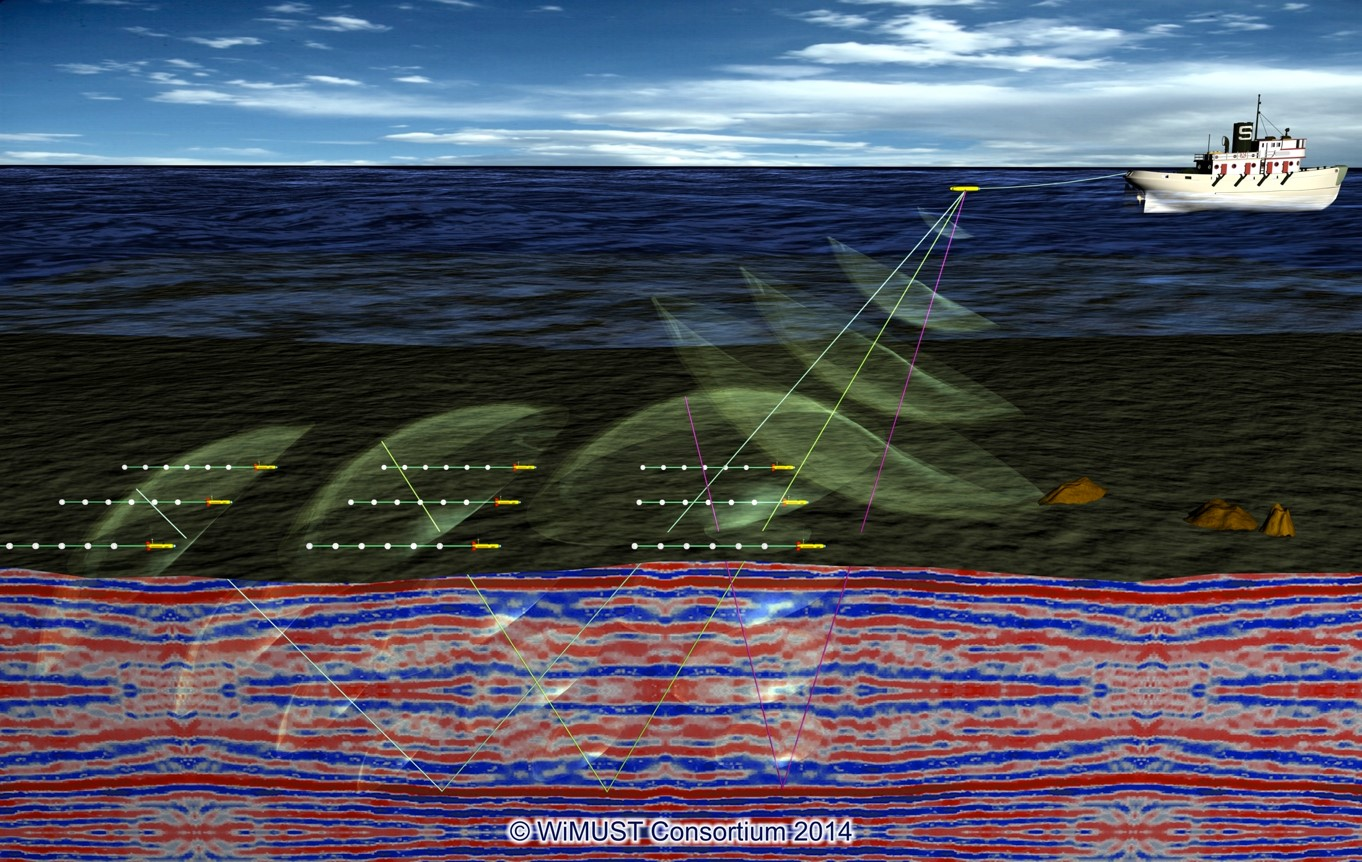
\includegraphics[width=0.5\textwidth]{Images/projects/WiMUST_project.jpg}
    \caption{Artist’s rendition of the WiMUST system for subbottom profiling with source-receiver decoupling}
    \label{fig:WiMUST_System}
\end{figure}

% \par A key-enabling element for the execution of such missions is the availability of advanced methods for cooperative motion planning that take explicitly into account temporal and spatial constraints, intrinsic vehicle limitations and energy minimisation requirements. 
% \par Some autonomous vehicle applications require groups of robots acting cooperatively. An application example that will greatly benefit from vehicle cooperation and that will be focus on this thesis is the control of groups of \acp{AUV} where the visibility is low and obstacles are not known in advance. The \acp{AUV} that together form a robot formation, can, for example, adapt better to unforeseen circumstances in the terrain by making better use of the larger environments that they can observe as the spatial distance between each \ac{AUV} can be varied.
% \par This project has evolved from earlier investigations on underwater mapping connected with the European R\&D Project "MORPH" Project~\cite{morph,aguiar2009cooperative} and the "WiMUST" Project~\cite{abreu2016widely} that Insitituto Superior Técnico was a part of. Figure~\ref{fig:morph} illustrates \acp{AUV} in operation on the Morph project.
% \par The "WiMUST" project, in particular, was composed by a small fleet of \acp{AUV} towing streamers with hydrophones to acquire sub-bottom profiling acoustic data.
% \par Recent advancements on the usage of \textit{Bernstein Polynomials} for control also appear to be advantageous,~\cite{cichella2018bernstein}, shows that it's possible to control a high number of vehicles with small computation time.

% \begin{figure}[h!]
%     \centering
%     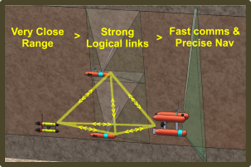
\includegraphics[width=0.5\textwidth]{Images/projects/Picture2.png}
%     \caption{Morph Project}
%     \label{fig:morph}
% \end{figure}
%     
% \begin{figure}[h!]
%     \centering
%     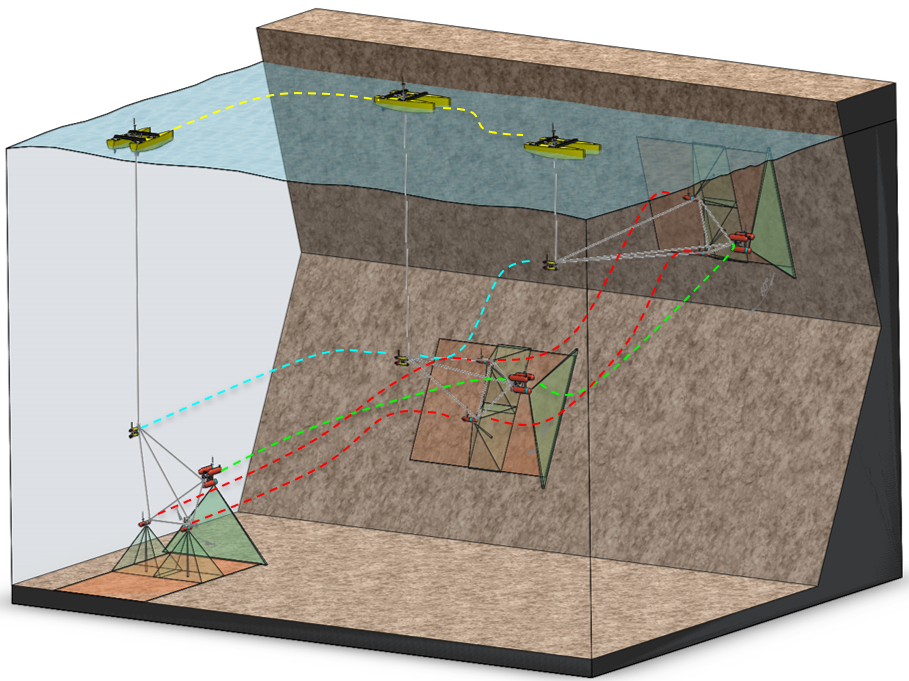
\includegraphics[width=0.6\textwidth]{Images/projects/Picture1.png}
%     \caption{Morph Project}
%     \label{fig:morph}
% \end{figure}


\section{Background}

\par The work discussed in this thesis focuses on motion planning for multiple cooperative vehicles. Motion Planning, as the name suggests, consists in planning motion for robots, such as mobile vehicles or robotic arms. Trajectory generation based on optimal control formulations will be used, specifically, to solve the motion planning problems. 
\par A trajectory is a time parameterized set of states of a dynamical system. These states can be position, their derivatives, heading, among others. The states and inputs are related to each other by a set of dynamic equations. When dealing with multiple vehicles, the trajectory optimisation problem takes into account the union of states and inputs of each vehicles such that the solution describes trajectories for all of the vehicles simultaneously.
\par As discussed in the previous section, numerical solutions to the trajectory generation problems must be sought. The numerical methods can be grouped into either direct methods or indirect methods. 
\par Indirect methods “use the necessary conditions of optimality of an infinite problem to derive a boundary value problem in ordinary differential equations”, the solutions of which must be found using analytic or numerical methods. 
\par Direct methods, on the other hand, are based on transcribing infinite optimal control problems into finite-dimensional \acp{NLP} using some kind of paramerisation (e.g., polynomial approximation or piecewise constant parameterization). They can be solved using ready-to-use NLP solvers (e.g. MATLAB) and do not require the computation of co-state and adjoint variables as indirect methods do.
\par The focus on the work of this thesis will be on the usage of Direct methods. Several parameterisation methods will be explored, such as peace-wise constants inputs, polynomials, and the usage of Bernstein polynomials.
\par When solving an optimisation problem, a model must be chosen for each vehicle. 
\par The states and inputs that describe a vehicle will depend on the choice of model for them. The choice of model to represent the \acp{AUV} will affect the dynamic equations that rule them.    which rule The Direct methods that will be tested will operate trajectories for be operated on different vehicle models, such as the Medusa Model \cite{abreu2016medusa} or a simpler Dubin's car \cite{wiki:dubincar}.

%\par The work discussed in this thesis emphasises in the use of motion planning for multiple cooperative vehicles. Motion Planning, as the name suggests, consists in planning motion for robots, such as mobile vehicles or robotic arms. The choice of control law, i. e., the input which is provided to a robot, will result in a motion which is optimal according to a certain criteria. This criteria could be, for example, minimising time or consumed fuel. Formulisation of such a problem is known as an optimal control problem.
%\par There are two main families of techniques for solving optimal control problems: direct methods and indirect methods.
%\par In an indirect method, the calculus of variations is employed to obtain the first-order optimality conditions. These conditions result in a two-point (or, in the case of a complex problem, a multi-point) boundary-value problem.

% https://math.stackexchange.com/questions/946343/optimal-control-difference-between-indirect-direct-approaches
%\par Direct methods in optimal control convert the optimal control problem into an optimisation problem of a standard form and then using a nonlinear program to solve that optimisation problem. 
%\par In direct approaches the optimal control problem is transfonned into a nonlinear
%programming problem.
%\par In a direct method, the state or the control, or both, are paramaterized in order to create an appropriate function approximation (e.g., polynomial approximation or piecewise constant parameterization). Simultaneously, the cost functional is approximated as a cost function. Then, the coefficients of the function approximations are treated as optimisation variables and the problem is "transcribed" to a nonlinear optimisation problem.
%
%\par A path is a parameterized curve, which is a function that maps a segment $[a,b]$ to $\mathbb{R}^3$. If the parameter of path $p$ is time or a function of time, the map $t\mapsto p(t)$ is called a trajectory.
%\par \ac{PF} refers to the problem of making vehicles converge to and follow a path with no explicit temporal schedule while \ac{TT} is the problem of making a vehicle track a trajectory such that both spacial and temporal schedules are satisfied simultaneously.
%\par Motion Planning consists in the design of trajectories for different kinds of systems that can later be tracked.
%\par A trajectory is the path that an object with mass in motion follows through space as a function of time. Trajectory tracking is the 
%\par The objective of motion planning is to find a trajectory to be tracked by a robot in an optimal way, based on a "cost function".
%
%\par Once decided what kind of parameterization will be used, the next step is to choose what model to represent the vehicle. Different models to represent vehicles exist such as a Dubin's car, Medusa Model.
% \par There are two main strategies for motion planning, one is \ac{TT} and the other is \ac{PF}. The first requires a vehicle to follow a path parameterized in space and time, whereas the latter only requires the vehicle to follow a path parameterized in space. Regardless of the strategy, the resulting evirnomental and dynamic constraints are met. Environmental constraints may include inter vehicular constraints, obstacle avoidance. Dynamic constraints include respecting maximum torque, acceleration, velocity and others for each vehicle.



\section{Objectives}


\par The work presented in this thesis focuses on the usage of Direct Methods.
\par There are several direct methods for trajectory optimisation, for example, single and multiple shooting, collocation and quadratic programming. However, polynomial methods based on Bezier curves are particularly advantageous because they have favourable geometric properties which allow the efficient computation of the minimum distance between trajectories. As the complexity of the polynomials increases, the solutions converge to the optimal.
\par The cost can be constructed based on several criteria such as time and consumed energy. For \textit{cooperative} motion planning, the cost will have to be constructed differently because it will have to take into account the motion of the multiple vehicles at once, in particular, possible inter-vehicle collision.
\par In practice, some of the objectives of this work include
\begin{itemize}
    \item test some methods for obstacle avoidance
    \item compare some different parameterization methodoligies
    \item analize the complexity of increasing order and number of vehicles
    \item test viability for non differentially flat systems
    \item test the usage of log barrier functions may help with speedinng up the optimisation process because they reduce the number of constraints by placing them in the cost function.
\end{itemize}


\section{Thesis Outline}

% to use refs: \ref{chap:available_methods} try \Cref{} too. it works for more than just  chapters
\par In chapter \ref{chap:theory}, an overview of the different available numerical methods for the motion planning for a single vehicle will be presented. \todo{exapnd}
\par In chapter \ref{chap:autonomousvehiclemodels}, an overview of different vehicle models is presented. \todo{expand}
\par In chapter \ref{chap:implementation}, a discussion of the code structure is discussed, along with the choice of optimisation algorithms. \todo{exapnd}
\par In chapter \ref{chap:results}, some results are presented. \todo{exapnd}
\par In chapter \ref{chap:conclusion}, the conclusion is made. \todo{exapnd}

This will be followed, in chapter , by application examples for a double integrator in 1 and 2 dimensions that capture the dynamics of a single vehicle. In chapter , some considerations for the control of multiple cooperative vehicles will be presented. The report will be concluded with a final overview of the different methods considered and a plan for the project's work will be defined.
